\section{Derivation of an Equivalent Quantum Graph Problem} \label{sec:ScalarDerivation}
In this section we demonstrate how system of the form \eqref{eq:SingularWaveEqnQGProblem} is obtained from \eqref{eq:SingularScalarWaveEqn}:
\begin{theorem} \label{thm:ScalarDerivation-Theorem}
	The problem \eqref{eq:SingularScalarWaveEqn} is equivalent to the problem \eqref{eq:SingularWaveEqnQGProblem}.
\end{theorem}
Section \ref{ssec:Scalar-QGDerivation} provides the proof of theorem \ref{thm:ScalarDerivation-Theorem}, and will setup our discussion revolving around the methods we employ for solving \eqref{eq:SingularWaveEqnQGProblem} in section \ref{sec:ScalarDiscussion}.
To do so, we will need to provide the reader with an intuitive understanding, stemming from the analysis of section \ref{sec:3DGradSobSpaces}, of the space $\tgradSob{\ddom}{\dddmes}$.
Upon deriving the quantum graph problem \eqref{eq:SingularWaveEqnQGProblem}, we will elaborate on its link to our variational problem in the context of Strauss extensions in section \ref{ssec:ExtendedSpaces}.

\subsection{Geometric Interpretation} \label{ssec:3DGradGeometric}
The intuition behind the form of the tangential gradients (and gradients of zero) with respect to the various measures $\lambda_{jk}, \ddmes, \nu$, and $\dddmes$ can be summarised with the colloquial phrase ``tangential gradients only reflect behaviour that the measure can see".
Let us be more precise, and first consider the measure $\lambda_{jk}$ for a fixed $I_{jk}$ and the associated gradients of zero and tangential gradients.
Suppose that we have a (sufficiently smooth) function $u$ defined on $\ddom$ that satisfies $u=0$ (or any constant value) on $I_{jk}$, from the perspective of $\lambda_{jk}$ this $u$ is the zero function,\footnote{more precisely, $u$ is represented by the zero function in $\ltwo{\ddom}{\lambda_{jk}}$.} regardless of whether $u$ is zero on the whole of $\ddom$ or not.
So despite $u=0$ in $\ltwo{\ddom}{\lambda_{jk}}$, it can have any profile in the direction $n_{jk}$ \emph{as it crosses} $I_{jk}$ and thus any kind of (reasonable) behaviour in the rest of $\ddom$ --- this is schematically illustrated in figure \ref{fig:Diagram_GradZeroIllustrations}.
\begin{figure}[b!]
	\centering
	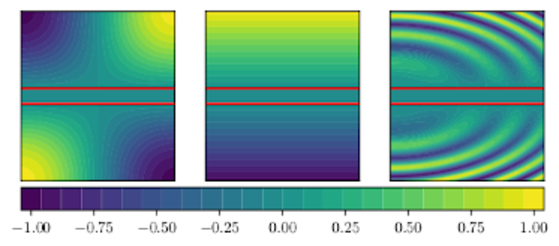
\includegraphics[scale=1.0]{Diagram_GradZeroIllustrations-Scaled.pdf}
	\caption{\label{fig:Diagram_GradZeroIllustrations} Examples illustrating how non-zero gradients of zero can arise, with the region between the red lines representing an edge $I_{jk}$, which has been thickened so one can view the function values along this edge. Despite each of the functions appearing constant along the edge $I_{jk}$, and thus constant to the measure $\lambda_{jk}$, the function is changing in the direction $n_{jk}$ as it crosses $I_{jk}$ and it's behaviour ``off the edge" is unknowable from the perspective of $\lambda_{jk}$. }
\end{figure}
Indeed, the measure $\lambda_{jk}$ is unable to deduce whether (for $x\in I_{jk}$) $u(x+hn_{jk})$ is different from $u(x)$ for $h\neq0$, given the only information it can have about $u$ are its values on $I_{jk}$.
Consequentially, $\lambda_{jk}$ can have no concept of $\pdiff{u}{n_{jk}}$ --- changing the profile of $u$ across the edge $I_{jk}$ does not change $u$ on $I_{jk}$, and consequentially the component of any ``gradient" directed along $n_{jk}$ corresponds to no change in the function $u$ from the perspective of $\lambda_{jk}$, making this component a gradient of zero.
In contrast, the measure $\lambda_{jk}$ can evaluate expressions like $u(x+he_{jk})-u(x)$ --- that is, changes in the function along $I_{jk}$ are detected by the measure $\lambda_{jk}$.
Such changes correspond to $\pdiff{u}{e_{jk}}$ being non-zero, and thus we find that tangential gradients are directed along $e_{jk}$ (and provide a ``derivative" in this direction too).
This also highlights the reason for defining the gradients of zero and tangential gradients as in section \ref{sec:BorelMeasSobSpaces} --- given a tangential gradient $\ktgrad_{\lambda_{jk}}u$, $\lambda_{jk}$ can reconstruct the function $u$ along the edge $I_{jk}$, but cannot determine what $u$ is doing across $I_{jk}$.
Ergo, every function has a gradient that is unique up to a gradient of zero, because there is no way for $\lambda_{jk}$ to determine what $u$ looks like across (and thus outside of) $I_{jk}$.

The above story is similar when considering the tangential gradient of $u$ with respect to the measure $\nu$.
Here, the ``view" of the measure is even more restricted, only being able to view the value of $u$ at the vertices, which are a set of isolated points in $\ddom$.
As such, there is no way for the measure $\nu$ to reconstruct any kind of sensible gradient --- there are no ``nearby" function values $u\bracs{v_j + h x}, x\neq 0$ to compare the value of $u\bracs{v_j}$ to.
The result is corollary \ref{cory:NuTangGradChar}, any gradient must be a gradient of zero, because as far as $\nu$ is concerned, there is no visible change in $u$ in any neighbourhood of $v_j$.
Then, given that $\dddmes$  is just the sum of the measures $\ddmes$ and $\nu$, we find that $\ktgrad_{\dddmes}u$ inherits the behaviours from $\ddmes$ and $\nu$.

\subsection{Derivation of the system \eqref{eq:SingularWaveEqnQGProblem}} \label{ssec:Scalar-QGDerivation}
We can now provide an argument for the proof of theorem \ref{thm:ScalarDerivation-Theorem}, that is how a system of the form \eqref{eq:SingularWaveEqnQGProblem} arises from \eqref{eq:SingularScalarWaveEqn}.
Take any $\varphi\in\csmooth{\sqbracs{0,l_{jk}}}$ and let $\phi\in\psmooth{\ddom}$ be such that $\phi\circ r_{jk} = \varphi$ on $\sqbracs{0,l_{jk}}$, with $\supp\phi\cap\graph\subset I_{jk}^{\circ}$.
Recall that the change of variables $r_{jk}$ is affine (see \eqref{eq:EdgeParameterisation}), so in particular this change of variables is invertable.
Testing against such $\phi$ in \eqref{eq:SingularScalarWaveEqn-VariationalForm}, combined with the fact that $\dddmes$ is a sum of the edge measures and point masses at the vertices, and that $\tgrad_{\dddmes}u=\tgrad_{\lambda_{jk}}u$ on the edge $I_{jk}$, equation \eqref{eq:SingularScalarWaveEqn-VariationalForm} implies
\begin{align*}
	0 &= \integral{\ddom}{ \bracs{\tgrad_\ddmes u \cdot \overline{\tgrad\phi} - \omega^2 u\overline{\phi}} }{\ddmes}
	= \integral{I_{jk}}{ \bracs{\tgrad_{\lambda_{jk}}u \cdot \overline{\tgrad\phi} - \omega^2 u^{(jk)}\overline{\phi}} }{\lambda_{jk}} \\
	&= \integral{I_{jk}}{ \clbracs{ \bracs{\bracs{u^{(jk)}}' + \rmi\qm_{jk} u^{(jk)}}\bracs{\overline{\phi}' - \rmi\qm_{jk} \overline{\phi} } - \omega^2 u^{(jk)}\overline{\phi} } }{\lambda_{jk}}.
\end{align*}
Now using the change of variables $r_{jk}$ and denoting $\tilde{u}^{(jk)} = u^{(jk)} \circ r_{jk}$, we arrive at
\begin{align*}
	0 &= \int_{0}^{l_{jk}} \bracs{\bracs{\tilde{u}^{(jk)}}' + \rmi\qm_{jk} \tilde{u}^{(jk)}}\bracs{\overline{\varphi}' - \rmi\qm_{jk} \overline{\varphi} } - \omega^2 \tilde{u}^{(jk)}\overline{\varphi} \ \md y. \\
	\implies
	\int_{0}^{l_{jk}} \bracs{\tilde{u}^{(jk)}}'\overline{\varphi}' \ \md y &=
	\int_{0}^{l_{jk}} \clbracs{ \omega^2\tilde{u}^{(jk)} + 2\rmi\qm_{jk}\bracs{\tilde{u}^{(jk)}}' + \bracs{\rmi\qm_{jk}}^2\tilde{u}^{(jk)} } \overline{\varphi} \ \md y.
\end{align*}
This holds for all $\varphi\in\csmooth{\sqbracs{0,l_{jk}}}$, and thus implies that $\tilde{u}^{(jk)}$ is twice (weakly) differentiable along $\sqbracs{0,l_{jk}}$.
Furthermore, we then obtain the (strong) equation
\begin{align*}
	-\bracs{\diff{}{y} + \rmi\qm_{jk}}^2 \tilde{u}^{(jk)} &= \omega^2 \tilde{u}^{(jk)}, \quad y\in\sqbracs{0,l_{jk}}.
\end{align*}

Now we turn our attention to the derivation of the vertex conditions.
Fix a vertex $v_j\in \vertSet$, and consider functions $\phi\in\psmooth{\ddom}$ with $\supp\phi\cap\graph\subset \mathcal{J}(v_j)\setminus\clbracs{v_j}$ (that is, smooth functions that are only non-zero on $\graph$ close to the vertex $v_j$).
Using the change of variables $r_{jk}$ on each edge and writing $\tilde{u}^{(jk)} = u^{(jk)} \circ r_{jk}$, $\varphi_{jk} = \phi\circ r_{jk}$ for each $k\con j$, we can work from \eqref{eq:SingularScalarWaveEqn-VariationalForm} to obtain
\begin{align*}
	0 &= \sum_{k: \ k\con j} \integral{I_{jk}}{ \bracs{ \tgrad_\ddmes u \cdot \overline{\tgrad\phi} - \omega^2 u\overline{\phi} } }{\lambda_{jk}} 
	+ \integral{\ddom}{ \bracs{ \tgrad_{\dddmes}u\cdot\overline{\tgrad_{\dddmes}\phi}-\omega^2 u\overline{\phi} } }{\massMes} \\
	&= \sum_{k: \ k\con j} \int_{0}^{l_{jk}} \clbracs{ \bracs{\bracs{\tilde{u}^{(jk)}}' + \rmi\qm_{jk} \tilde{u}^{(jk)}}\bracs{\overline{\varphi}_{jk}' - \rmi\qm_{jk} \overline{\varphi}_{jk} } - \omega^2 \tilde{u}^{(jk)}\overline{\varphi}_{jk} } \ \md y \\
	&\qquad + \alpha_j\left.\bracs{ \tgrad_{\dddmes}u\cdot\overline{\tgrad_{\dddmes}\phi}-\omega^2 u\overline{\phi} }\right\vert_{v_j} \\
	&= \sum_{k: \ k\con j} \int_{0}^{l_{jk}} \clbracs{ \bracs{\bracs{\tilde{u}^{(jk)}}' + \rmi\qm_{jk} \tilde{u}^{(jk)}}\bracs{\overline{\varphi}_{jk}' - \rmi\qm_{jk} \overline{\varphi}_{jk} } - \omega^2 \tilde{u}^{(jk)}\overline{\varphi}_{jk} } \ \md y
	 - \alpha_j \omega^2 u\bracs{v_j}\overline{\phi}\bracs{v_j}.
\end{align*}
Here we have used the fact that $\tgrad_{\dddmes}u\bracs{v_j}=0$ (see section \ref{sec:3DGradSobSpaces}).
Given that (from our considerations along the edges) $u$ is twice differentiable on each $I_{jk}$, and $\phi$ is zero at every vertex except $v_j$, it follows that
\begin{align*}
	\alpha_j\omega^2 u\bracs{v_j}\overline{\phi}\bracs{v_j} 
	&= - \sum_{k: \ k\con j} \int_{0}^{l_{jk}} \bracs{ \bracs{\diff{}{x} + \rmi\qm_{jk}}^2 \tilde{u}^{(jk)} +\omega^2 \tilde{u}^{(jk)} }\overline{\varphi}_{jk} \ \md y \\
	&\qquad + \sum_{k: \ k\con j}\overline{\varphi}_{jk}\bracs{v_j}\bracs{\pdiff{}{n} + \rmi\qm_{jk}}\tilde{u}^{(jk)}\bracs{v_j} \\
	&= \overline{\phi}\bracs{v_j}\sum_{k: \ k\con j}\bracs{\pdiff{}{n} + \rmi\qm_{jk}}\tilde{u}^{(jk)}\bracs{v_j}. \labelthis\label{eq:DerivationVertexConditionWeak}
\end{align*}
Given that \eqref{eq:DerivationVertexConditionWeak} holds for every smooth $\varphi$, and that $\varphi_{jk}\bracs{v_j}=\phi\bracs{v_j}$, we arrive at the condition
\begin{align*}
	\alpha_j\omega^2 u\bracs{v_j} &= \sum_{j\con k}\bracs{\pdiff{}{n} + \rmi\qm_{jk}}\tilde{u}^{(jk)}\bracs{v_j}.
\end{align*}

Repeating the argument for each $v_j\in \vertSet$ then provides us with a condition of this form at each vertex.
One should note the presence of $\omega^2$ in this equation, so this is not a Kirchoff condition on the derivatives of the edge functions $u^{(jk)}$, and indicates that the problem we have arrived at is defined through an operator acting in an extended space, as mentioned in section \ref{ssec:DiffOpsOnGraphs}.
The result of theorem \ref{thm:dddmesTangGradImplication} tells us that functions $u\in\gradSobQM{\ddom}{\dddmes}$ are also continuous at each vertex $v_j$, and thus the following problem (precisely \eqref{eq:SingularWaveEqnQGProblem}) has been derived:
\begin{subequations}
	\begin{align*}
		-\bracs{\diff{}{y} + \rmi\qm_{jk}}^2 u^{(jk)} &= \omega^2 u^{(jk)}, \quad &y\in\sqbracs{0,l_{jk}}, \ \forall I_{jk}\in\edgeSet, \tag{\eqref{eq:SingularWaveEqnQGProblem-1} restated} \\
		u \text{ is continuous at } & v_j, \quad &\forall v_j\in\vertSet,  \tag{\eqref{eq:SingularWaveEqnQGProblem-2} restated} \\
		\sum_{j\con k}\bracs{\pdiff{}{n} + \rmi\qm_{jk}}u^{(jk)}\bracs{v_j} &= \omega^2\alpha_j u\bracs{v_j}, \quad &\forall v_j\in\vertSet, \tag{\eqref{eq:SingularWaveEqnQGProblem-3} restated}
	\end{align*}
\end{subequations}
where we henceforth drop the overhead tilde notation and simply write $u^{(jk)}$ for brevity (appealing to the obvious association between $u^{(jk)}$ and $\tilde{u}^{(jk)}$).
As will be made clear in the discussion that follows, the quantum graph problem \eqref{eq:SingularWaveEqnQGProblem} is much easier to handle (than \eqref{eq:SingularScalarWaveEqn}) analytically and numerically thanks to the utility of the $M$-matrix.

Now that we have obtained the system \eqref{eq:SingularWaveEqnQGProblem}, we can affirm our interpretation of the coupling constants $\alpha_j$ as the (limit of the) ratio of vertex volume $V_{\mathrm{vertex}}$ to edge volume $V_{\mathrm{edge}}$ that was described in section \ref{ssec:Intro-ThinStructures}.
As can clearly be seen from \eqref{eq:SingularWaveEqnQGProblem-3}, when $\alpha_j$ is non-zero and finite, we obtain Wentzell conditions between the incoming derivatives to the vertex $v_j$.
This is precisely the boundary condition we would obtain in the zero-thickness limit for the (Neumann) Laplacian on a thickened graph, provided the ratio $\frac{V_{\mathrm{vertex}}}{V_{\mathrm{edge}}}\rightarrow\alpha_j$ as the thickness of the structure tended to zero.
Moreover, notice that if $\alpha_j=0$ in \eqref{eq:SingularWaveEqnQGProblem-3}, we obtain an exact Kirchoff condition at the vertex $v_j$, along with continuity of the incoming edge functions --- precisely the case when $V_{\mathrm{vertex}}\ll V_{\mathrm{edge}}$.
Finally, if one divides through by $\alpha_j$ in \eqref{eq:SingularWaveEqnQGProblem-3} and takes a formal limit as $\alpha_j\rightarrow\infty$, the resulting system imposes homogeneous Dirichlet boundary conditions on the solution $u$ at $v_j$ --- corresponding to the conditions obtained in the limiting case $V_{\mathrm{vertex}}\gg V_{\mathrm{edge}}$.
We can also predict the resulting problems of thickened graphs that possess a mixture of vertex and edge volumes; that is when a thickened graph $\mathcal{G}_{\delta}$ of $\graph$ is such that $V_{\mathrm{edge}}\bracs{\delta}$ is the same for every (thickened) edge, yet the scaling of the volume of the thickened vertices $V_{v_j}\bracs{\delta}, v_j\in\vertSet$ with $\delta$ changes between vertices.
Letting $\alpha_j = \lim_{\delta\rightarrow0}\frac{V_{v_j}}{V_{\mathrm{edge}}}$ (where we formally allow $\alpha_j=\infty$) for each $v_j$, our consideration of singular measures and the variational problem \eqref{eq:SingularScalarWaveEqn} predicts that the resulting system will be realisable as the following quantum graph problem:
\begin{subequations}
	\begin{align*}
		-\bracs{\diff{}{y} + \rmi\qm_{jk}}^2 u^{(jk)} &= \omega^2 u^{(jk)}, \quad & y\in\sqbracs{0,l_{jk}}, \ \forall I_{jk}\in\edgeSet, \\
		u \text{ is continuous at } & v_j, \quad &\forall v_j\in\vertSet, \\
		\sum_{j\con k}\bracs{\pdiff{}{n} + \rmi\qm_{jk}}u^{(jk)}\bracs{v_j} &= \omega^2\alpha_j u\bracs{v_j}, \quad &\forall v_j\in\vertSet, \ \alpha_j\in\bracs{0,\infty}, \\
		\sum_{j\con k}\bracs{\pdiff{}{n} + \rmi\qm_{jk}}u^{(jk)}\bracs{v_j} &= 0, \quad &\forall v_j\in\vertSet, \ \alpha_j = 0, \\
		u\bracs{v_j} &= 0, \quad &\forall v_j\in\vertSet, \ \alpha_j = \infty.
	\end{align*}
\end{subequations}
We also remark that, for a graph with $\alpha_j<\infty$ for every $v_j$, our approach via the $M$-matrix (section \ref{sec:ScalarDiscussion}) for determining the spectrum of the above problem can be employed.

\subsection{The relation between $\tgradSob{\ddom}{\dddmes}$ and extended spaces} \label{ssec:ExtendedSpaces}
As we have already discussed, the problem \eqref{eq:SingularWaveEqnQGProblem} coincides with the problems that arise in the zero-thickness limit of thin-structures.
Indeed, the system \eqref{eq:SingularWaveEqnQGProblem} corresponds to the operator $\mathcal{A}_{\mathrm{ext}}$ that acts in the \emph{extended space}
\begin{align*}
	\dom\mathcal{A}_{\mathrm{ext}} 
	&= \clbracs{ (u, \beta) \setVert u\in H^2\bracs{\graph}, \ u \text{ is continuous at each } v_j\in\vertSet, \ \beta_j=\alpha_j u(v_j) } \\
	& \subset L^2\bracs{\graph}\oplus\complex^{\abs{\vertSet}}.
\end{align*}
The element $\bracs{u,\beta}$ is a $\abs{\edgeSet}+\abs{\vertSet}$ ``vector" (more precisely, tuple) consisting of the edge functions $u^{(jk)}$, followed by the (scaled) vertex values $\beta_j$, which we shall write as
\begin{align*}
	\begin{pmatrix} u \\ \beta \end{pmatrix}
	&= \begin{pmatrix} \clbracs{u^{(jk)}}_{I_{jk}\in\edgeSet} \\ \clbracs{\beta_j}_{v_j\in\vertSet} \end{pmatrix}.
\end{align*}
The action of $\mathcal{A}_{\mathrm{ext}}$ defined as
\begin{align*}
	\mathcal{A}_{\mathrm{ext}} \begin{pmatrix} u \\ \beta \end{pmatrix}
	&= 
	\begin{pmatrix}
		\clbracs{-\bracs{\diff{}{y}+\rmi\qm_{jk}}^2 u^{(jk)}}_{I_{jk}\in\edgeSet} \\ 
		\clbracs{\sum_{j\con k}\bracs{ \pdiff{}{n} + \rmi\qm_{jk} }u^{(jk)}(v_j)}_{v_j\in\vertSet}
	\end{pmatrix},
\end{align*}
the space $L^2\bracs{\graph}\oplus\complex^{\abs{\vertSet}}$ is the extended space, and $\mathcal{A}_{\mathrm{ext}}$ the Strauss extension for the problem \eqref{eq:SingularWaveEqnQGProblem}.

The operators $\mathcal{A}_{\mathrm{ext}}$ and $-\laplacian_{\dddmes}^{\qm}$ possess the same eigenvalues and eigenfunctions by virtue of theorem \ref{thm:CharOfSobSpaces}.
If $\omega^2$, $u$ is an eigenpair of $-\laplacian_{\dddmes}^{\qm}$, then this eigenpair solves \eqref{eq:SingularWaveEqnQGProblem} by virtue of theorem \ref{thm:ScalarDerivation-Theorem}.
In particular we have that $u\in H^2\bracs{\graph}$ and is continuous through the vertices (as a consequence of theorem \ref{thm:CharOfSobSpaces}), so one has that $\bracs{u,\beta = \clbracs{\alpha_j u(v_j)}_{v_j\in\vertSet}}$ satisfies $\mathcal{A}_{\mathrm{ext}}\bracs{u,\beta} = \omega^2\bracs{u,\beta}$.
Conversely if $\omega^2, \bracs{u,\beta}$ is an eigenpair of $\mathcal{A}_{\mathrm{ext}}$, then $u\in\tgradSob{\ddom}{\dddmes}$ by theorem \ref{thm:CharOfSobSpaces} (it is continuous through the vertices and $H^1$ on the edges) and takes the values $u(v_j) = \alpha_j^{-1}\beta_j$ at the vertices.
The pair $omega^2, u$ also solves the system \eqref{eq:SingularWaveEqnQGProblem}, so by theorem \ref{thm:CharOfSobSpaces} also constitutes an eigenpair of $-\laplacian_{\dddmes}^{\qm}$.
A similar argument also extends to the situation where one considers $f\in L^2\bracs{\graph}\oplus\complex^{\abs{\vertSet}} \cong \ltwo{\ddom}{\dddmes}$ and solution to the problem $\mathcal{A}_{\mathrm{ext}}u=f$ and $-\laplacian_{\qm}^{\dddmes}u=f$. 
Here one follows a similar procedure to the proof of theorem \ref{thm:ScalarDerivation-Theorem}, realising that the problem $-\laplacian_{\qm}^{\dddmes}u=f$ can be written in the form \eqref{eq:SingularWaveEqnQGProblem}, except replacing $\omega^2 u$ with $f$ in \eqref{eq:SingularWaveEqnQGProblem-1} and $\omega^2\alpha_j u(v_j)$ with $\alpha_j f(v_j)$ in \eqref{eq:SingularWaveEqnQGProblem-3}.
The fact that $f\in\ltwo{\ddom}{\dddmes}$ is important here, as it provides enough regularity for $u$ to be an element of $H^2\bracs{\graph}$.

Our approach via singular measures has resulted in the immediate construction of the extended space \emph{and corresponding operator} one obtains in the zero-thickness limit of thin-structure problems.
Within the context of the acoustic approximation we already knew what these limits where, however our original formulation provides a method of defining this limiting problem by appealing to the geometry.
This also presents an opportunity we look to investigate going forward; the non-classical Sobolev spaces and variational problems provide us with a method of defining (up to isomorphism) the spaces and problems that may correspond to the --- presently unknown --- ``limits" of other thin-structure problems.